\section{Wstęp}
%Część ta~zawiera wstępne informacje o~realizowanym projekcie. Zebrano w~nim wszystko to~co było dostępne zanim student przystąpił do~realizacji informatycznej części projektu. Opisano stanowisko laboratoryjne na~którym powstał projekt.

%\subsection{Geneza}
Tematem projektu, którego dotyczy ta praca jest: „Projekt i~realizacja stanowiska laboratoryjnego do badania zależności czasowych w~sieci EtherCAT". Zagadnienia związane z~tworzeniem oprogramowania dla sterowników przemysłowych są dla autora niezwykle interesujące, a zrealizowany projekt miał na~celu dalsze pogłębienie jego wiedzy z tego zakresu. Wyboru tego konkretnego tematu autor dokonał, ponieważ protokół EtherCAT jest jeszcze nowością i według wielu źródeł stanowi przyszłość branży informatyki przemysłowej \cite{art1, art2}, a~praca nad tym tematem wydaje się być pomocna i~wartościowa w przyszłej pracy zawodowej lub na~ewentualnym dalszym etapie kształcenia.

%\subsection{Temat}
%System sterowania i wizualizacji pracy robota 3D. \\
Głównymi celami pracy było napisanie oprogramowania dla sterownika przemysłowego Siemens S7-300 oraz stworzenie graficznej prezentacji pracy modelu Robota~3D takiego jak na~Rysunku~\ref{robot}.
Dodatkowym elementem pracy inżynierskiej zrealizowanej przez autora jest element pozainformatyczny, a mianowicie zbudowanie magazynu, z~którym robot będzie współpracował. Wyżej wspomniany magazyn po zakończeniu projektu posłuży jako pomoc dydaktyczna do~ćwiczeń laboratoryjnych.
%\begin{figure}[!htb] \centering 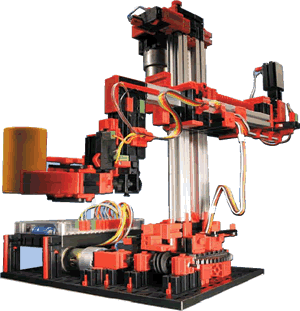
\includegraphics[width=0.4\textwidth]{obrazki/Fischertechnik3DRobot.png} \caption{Robot 3D firmy Fischertechnik} \label{robot} \end{figure}

\subsection{Stanowisko laboratoryjne}
%\begin{figure}[!htb] 	\centering 	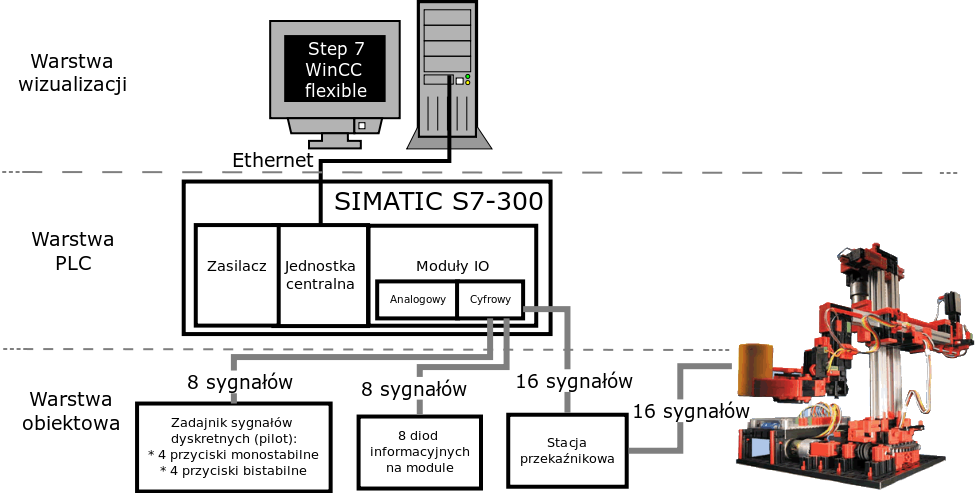
\includegraphics[width=0.99\textwidth]{obrazki/schemat.png} 	\caption{Schemat stanowiska} \label{schemat} \end{figure} 
Na potrzeby realizacji projektu wykorzystano dwa różne istniejące stanowiska laboratoryjne, które składały się odpowiednio~z:
\begin{table}[!htb]
\begin{center}
\begin{tabular}{| p{0.5\textwidth} || p{0.5\textwidth} |}\hline
Stanowisko typu CX & Stanowisko typu CP   \\\hline
\begin{enumerate}
\item 2~silniki AM3021-0C00-0000,
\item Wyspa EK1100 z~zestawem modułów~IO,
\item Napęd serwomechnizmów AX5203 (2~osiowy napęd),
\item Komputer przemysłowy C6925,
\item Zasilacz.
\end{enumerate}
&
\begin{enumerate}
\item 2~silniki AM3021-0C00-0000,
\item Wyspa EK1100 z~zestawem modułów IO,
\item Napęd serwomechnizmów AX5203 (2~osiowy napęd),
\item Modułowy komputer przemysłowy CX1020,
\item Zasilacz.
\end{enumerate}
\\\hline                                            
\end{tabular}
\end{center}
\vspace*{-6mm}
  \caption{Dostępne stanowiska laboratoryjne}
	\label{in}
\end{table}

\subsubsection{Sterownik PLC}
Sterownik PLC wykorzystywany do realizacji projektu był wyposażony w następujące moduły:
\begin{enumerate}
\item SIMATIC S7-300, Jednostka centralna S7-300 CPU 315F-2 PN/DP,
\item SIMATIC S7-300, Zasilacz PS 307,
\item SIMATIC S7-300, Wejścia/Wyjścia cyfrowe SM 323,
\item SIMATIC S7-300, Wejścia/Wyjścia analogowe SM 334.
\end{enumerate}
%\begin{figure}[!htb] 	\centering 	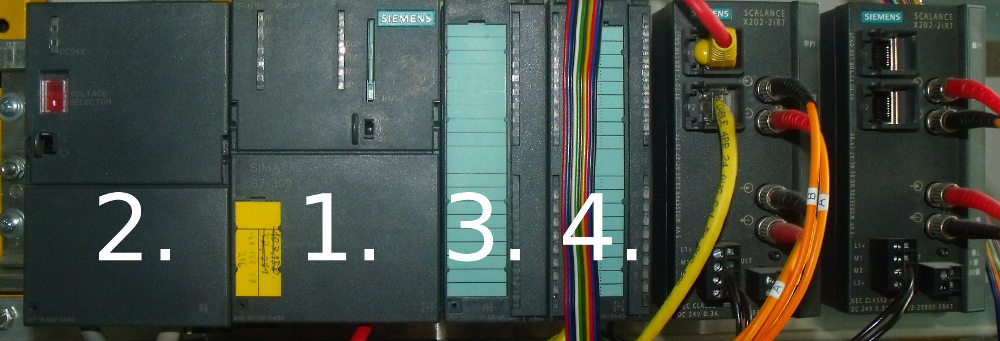
\includegraphics[width=0.75\textwidth]{obrazki/sterownik.png} 	\caption{Siemens SIMATIC S7-300} \end{figure}
\indent
\indent Sterownik podłączony jest do sieci lokalnej Ethernet w~laboratorium, więc komunikacja z~nim odbywa się tak samo jak z~każdym innym urządzeniem sieciowym. Podstawy programowania i korzystania ze sterowników autor poznał zapoznając się z odpowiednią literaturą \cite{plc1,plc2,plc4,plc5,plc6}.
Konfigurację sterownika wraz z modułami przedstawia Rysunek~\ref{conf}.
%\begin{figure}[!htb] 	\centering 	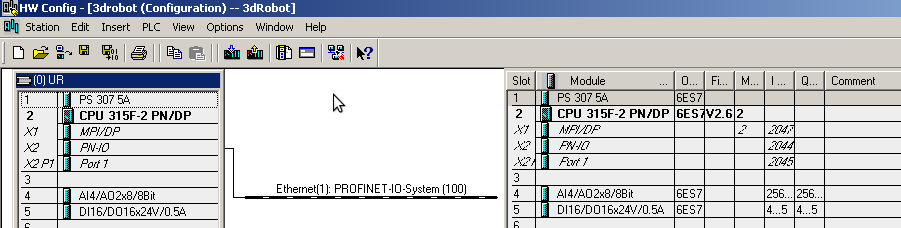
\includegraphics[width=0.75\textwidth]{obrazki/conf.png} \caption{Konfiguracja sterownika PLC} \label{conf} \end{figure}
\subsubsection{Komputer}
Projekt w całości był realizowany na laptopie autora, podłączanym do~sieci w~laboratorium. Na~komputerze uruchomiane były dwie maszyny wirtualne. Na~jednej zainstalowane było środowisko Step~7 do~programowania sterownika, a~na~drugiej WinCC flexible 2008 do~tworzenia i~uruchamiania wizualizacji. Wizualizacje tworzone w środowisku WinCC flexible są~dedykowane do~paneli operatorskich, jednak ta~stworzona przez autora na~potrzeby projektu była uruchamiana na komputerze za~pomocą runtime system.

!!!!!!!!
\subsection{•}
\subsection{Analiza tematu}
Analiza tematu polegała przede wszystkim na zapoznaniu się z~narzędziami programistycznymi do~tworzenia oprogramowania sterownika oraz wizualizacji.
W~wyniku analizy autor poznał podstawy języków: LAD~\cite{step1,step2,step3}, STL~\cite{step1,step2,step3}, FBD~\cite{step1,step2,step3}, GRAPH~\cite{step3}, SCL~\cite{scl1,scl2,scl3} i AWL do~tworzenia programu sterownika oraz VBScript do~tworzenia skryptów w~wizualizacji.
Poznanie tych podstaw pozwoliło dobrać język odpowiedni do~realizacji poszczególnych zadań.

\subsection{Założenia}
Oprogramowanie dla dostępnego stanowiska laboratoryjnego powinno zostać stworzone przy użyciu środowiska TwinCAT. Funkcjonalności robota wchodzące w~skład projektu, to:
\begin{itemize}
\item sterowanie ręczne z~pilota podłączonego bezpośrednio do~sterownika,
\item sterowanie ręczne z~wizualizacji,
\item sterowanie automatyczne, 
\item wizualizacja stanu stanowiska.
\end{itemize}
\indent
\indent Powyżej zostały wymienione założenia podstawowe, jednak autor nie wyklucza zrealizowania dodatkowych zadań, które nie zostały zamieszczone w~pierwotnej koncepcji realizacji projektu.

\subsection{Plan pracy}
Realizacja projektu została podzielona na następujące etapy:
\begin{itemize}
\item Zapoznanie się ze sterownikami Beckhoff oraz oprogramowaniem TwinCAT,
\item Zapoznanie się z dostępnymi serwonapędami Beckhoff,
\item Projekt i realizacja stanowiska,
\item Przygotowanie stanowiska do współpracy z systemem wizualizacji,
\item Testowanie i uruchamianie,
\item Przedstawienie projektu i~ewentualne korekty.
\end{itemize}
\indent
\indent Powyższy plan pracy stanowił dla autora wyznacznik kolejnych działań. Jednak powszechnie wiadomo, że w~praktyce poszczególne punkty są~wymienne i~wpływają na siebie wzajemnie.
